% DivaPreprocessing
\chapter{Preparation of the input files\label{Preprocessing}}

We describe in this chapter the tools to prepare the various input files presented in Chapter~\ref{chap:general}. If you already have the input files at your disposal, you way want to go directly to the next chapter.

\minitoc

\section{Creation of topography\label{sec:howtotopo}}
%---------------------------------------------------------

\index{Topography}
Topographies are necessary in two cases: first when you work in a vertical plane and want to interpolate several profiles from a cruise; second is when you need contour files at different depths to perform analysis. We describe here two techniques to get a topography file compatible with \diva.


\begin{center}
\fbox{
\begin{minipage}{0.9\textwidth}
\vspace{.25cm}
\textbf{Convention:} \diva works with the convention that depth are positive under the sea level. This is especially important when creating contours. \matlab\,tools provided with the software create topographies which respect this convention, but in case that you work with topography database that are not described in the following section,  
\vspace{.25cm}
\end{minipage}
}
\end{center}

\btips
A simple way to change the sign of a given column of a data file is to use the following command:
\begin{verbatim}
awk '{print $1,$2,-$3}' infile > outfile
\end{verbatim}
where \texttt{infile} is the old file and \texttt{outfile} the new one.

If you need to switch two columns of a file, type:
\begin{verbatim}
awk '{print $2,$1,$3}' infile > outfile
\end{verbatim}
\etips



\subsection{Method 1: conversion from GEBCO topography\label{sec:topogebco}}
%------------------------------------------------------

Download the complete, global GEBCO One-Minute Grid file (\file{90n90s180w180e.zip}) from \url{http://www.bodc.ac.uk/data/online_delivery/gebco/} and unzip it to obtain the file \file{GridOne.grd}. Download the software \texttt{GebcoCE\_GridOnly} as well and run it. 

\subsubsection{Select your area}
%-------------------------------

Select your region of interest (Fig.~\ref{fig:gebco1}), possibly slightly increased to make sure boundaries are well included in the topography. Then select {\tt File->Export Data->Gridded Data}. Chose Ascii longitude-latitude-depth (default). For the longitude range, use {\tt -180:180} for european seas. Note regions you possibly want to mask later by their coordinate ranges.  Use {\tt topo.gebco.asc} as output file name, into a directory where
you have your main climatological working place. Push {\tt OK} and be patient. (Fig. \ref{fig:gebco2}). 

\begin{figure}[htpb]
\centering
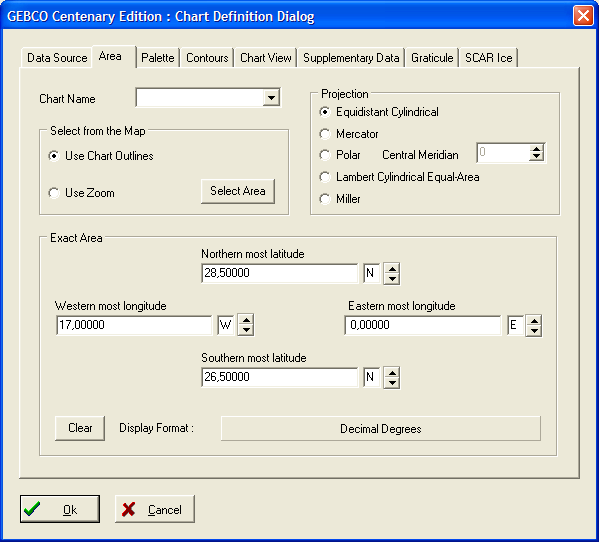
\includegraphics[width=.65\textwidth]{topoGEBCO2}
\caption{Area selection with software \texttt{GebcoCE\_GridOnly}.\label{fig:gebco1}}
\end{figure}


\begin{figure}[htpb]
\centering
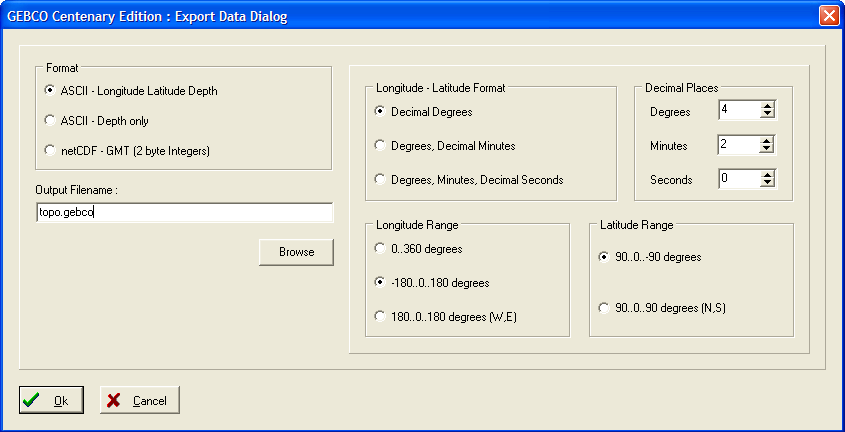
\includegraphics[width=.65\textwidth]{topoGEBCO3}
\caption{Data exportation with software \texttt{GebcoCE\_GridOnly}.\label{fig:gebco2}}
\end{figure}



%\subsubsection{Convert commas into dots}
%%---------------------------------------
%
%Depending on your installation, decimal numbers may be written with commas instead of points in GEBCO gridded file. In order to be compatible with \diva convention it is necessary to change the commas into points (see beginning of Chap. \ref{chap:general}).


\subsubsection{Convert the file into \texttt{gher} format}
%--------------------------------------------------------- 

%For the conversion, two possibilities are offered:
%\begin{enumerate}
%
%\item With the bash script \command{gebco2diva}: simply copy the files created by the extraction into the \directory{input} directory with the name \file{topo.gebco} and clean the header (i.e., eliminate lines of comments); the execution of \command{gebco2diva} will provide you with \file{topo.grd} and \file{TopoInfo.dat} in the \directory{output} directory.
%
%
%\item The second possibility consist in applying \matlab\, tool \file{diva\_topo\_gebco.m} on file \file{topo.gebco} in order to convert it into a \diva-usable topography.
%
%\end{enumerate}

Go into Cygwin (or into Linux mode) and place yourself in the main directory of your climatology production. You should have a big {\tt topogebco.asc} file on which you can apply

\begin{lstlisting}[style=Bash]
[charles@gher13 input] head -20 topogebco.asc
\end{lstlisting}

to see if the file was created correctly. You also should have a \command{gebcoprep} file. If not, copy the \file{gebcoprep.example} file as \command{gebcoprep}.

If you need to mask regions, edit \command{gebcoprep} and add lines as those put with {\tt \#awk} followed by {\tt \#mv bidon}. They should be self explaining and allow excluding regions that are defined by relationships between longitude and latitude. (Example: {\tt ($2 > 57.0+0.6*$1) {x=-10.} } means that regions where latitude is larger than \texttt{57+0.6*longitude} will be masked). Then execute \command{gepcoprep} and be {\bf very} patient when working on large domains. Normally you do not to repeat this step a lot of times.

Once you defined the regions to be masked in this way, execute \command{gebcoprep}. This will create a file
\file{./input/topo.gebco}, which you can have a look at with the \command{head} command.

Now you are ready to prepare the gridded topography \file{topo.grd} from which \diva will extract contours. To prepare it,
copy or move \file{./input/topo.gebco} into the diva working directory to have \file{divastripped/input/topo.gebco}.

The resolution of GEBCO is 1 minute. This might be much too fine for large scale analysis and you can run
{\tt gebco2diva} with optional arguments {\tt nx ny} to make a grid using only every {\tt nx} point in $x$ direction and {\tt ny} in $y$ direction. If for example you are interested in a \diva output resolution that is working at a 100 km scale, {\tt gebco2diva 15 15} would still provide a very fine topography with respect to the scales of interest.

Place yourself into the {\tt divastripped} directory. Once you executed {\tt gebco2diva} and a little patience for big files, you should find in {\tt divastripped/output} two files describing the gridded topography: {\tt topo.grd} and {\tt TopoInfo.data}. While the former is a binary file, the latter tells you (via {\tt cat ./output/TopoInfo.dat}) the topology of the grid.


You can further check the two files by copying them into the {\tt divastripped/input} directory and executing {\tt divacont} and {\tt divagnu}. If results seem right, you can save the files {\tt TopoInfo.data} and {\tt topo.grd} into your main data directory, to be used with {\tt divacont} on all levels defined by {\tt contour.depth}.

If everything is stable, you can erase {\tt topogebco.asc} and {\tt topo.gebco} to save disk space. 


\begin{figure}[htpb]
\centering
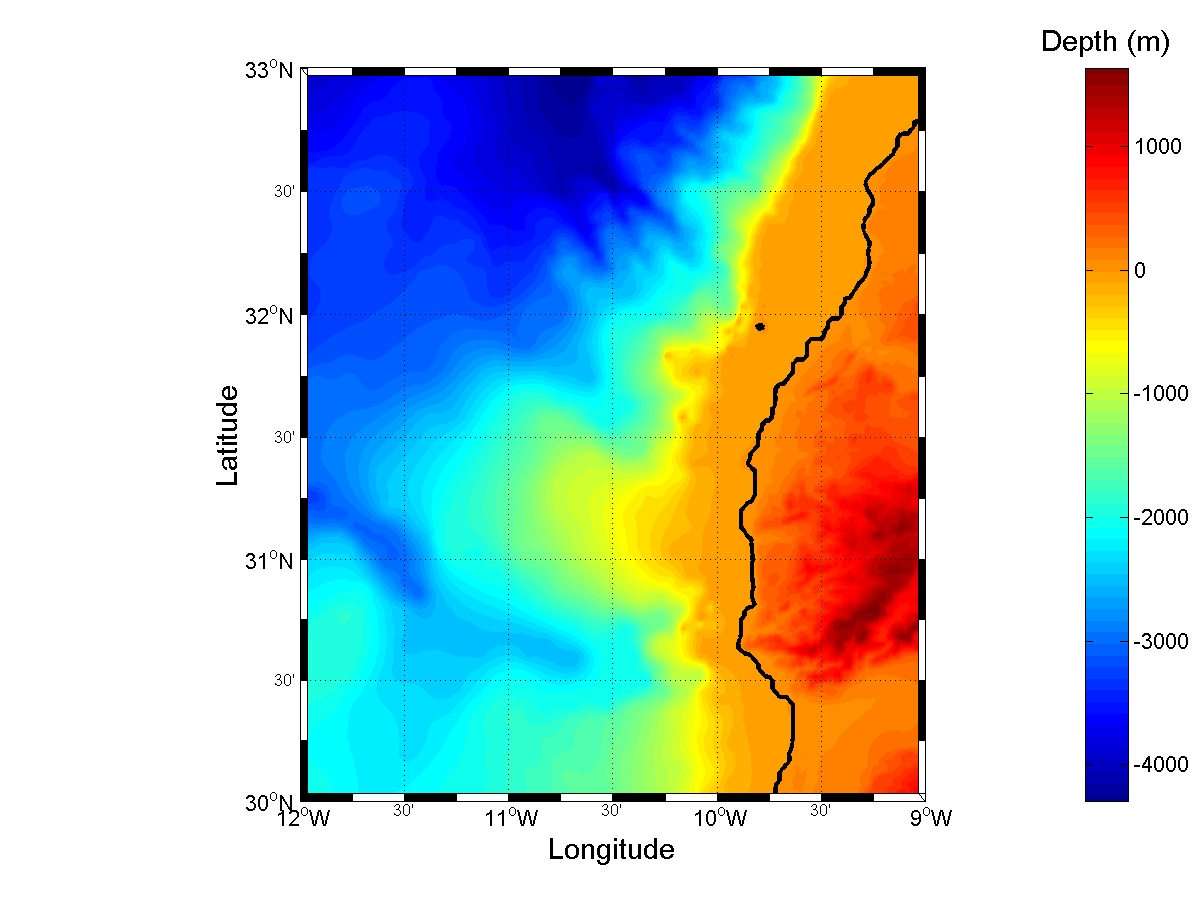
\includegraphics[width=.75\textwidth]{Ghir_topo_gebco}
\caption{Topography from GEBCO one-minute topography.\label{fig:topoGebco3}}
\end{figure}

\subsection{Method 2: conversion of data from Topography Extractor\label{sec:toponavy}}
%------------------------------------------------------------------

\subsubsection{Select your area}
%-------------------------------

Go to \url{https://idbms.navo.navy.mil/dbdbv/dbvquery.html}, select the area and spacing and download the corresponding file in \texttt{CHRTR ascii} format (Fig. \ref{fig:topoextract}). In this example we worked in the region delimited by $[9-12^{\circ}W\, \times\, 30-33^{\circ}N]$ (NW Africa) with a resolution of $0.01^{\circ}$ in both directions. 


\begin{figure}[htpb]
\centering
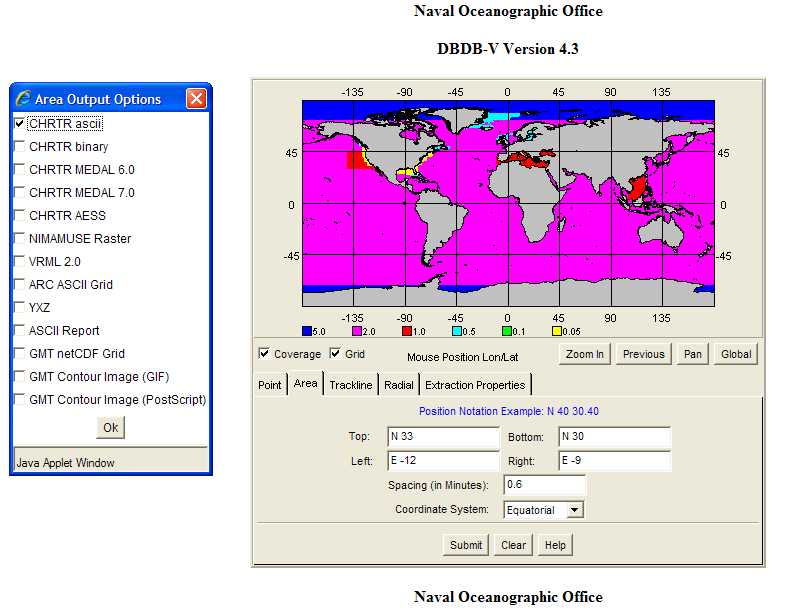
\includegraphics[width=.75\textwidth]{TopoNaval}
\caption{Topography extraction from the Naval Oceanographic Office website.\label{fig:topoextract}}
\end{figure}

If the web server is not operational, you can also access this database at \url{http://ferret.pmel.noaa.gov/NVODS/servlets/}
Then select your dataset by clicking on "\textsl{by Dataset Name}" and chose 
"\textsl{NAVAL OCEANOGRAPHIC OFFICE Bathymetry/Topography 5min resolution}".

Mark the topography box and click on "\textsl{Next}" (Fig. \ref{fig:nvods1}).\\
Delimit your region and select "ASCII file" as output (Fig. \ref{fig:nvods2}). 


\begin{figure}[htpb]
\centering
\subfigure[]{
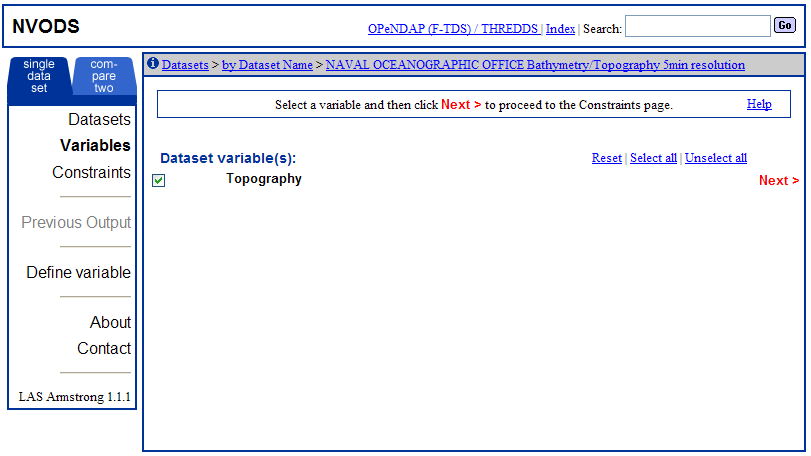
\includegraphics[width=.7\textwidth]{TopoNVODS1}
\label{fig:nvods1}
}

\subfigure{
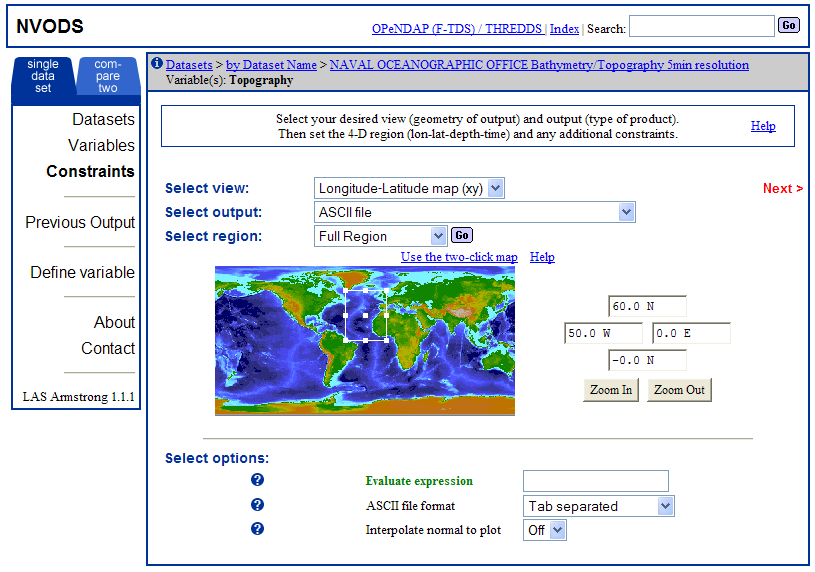
\includegraphics[width=.7\textwidth]{TopoNVODS2}
\label{fig:nvods2}
}
\caption{Topography extraction from NVODS.}
\end{figure}


Put the \file{.asc} file into \directory{divastripped/input/} with the name \file{topo.asc} and execute \command{dbdb2diva} in the shell. You will get \file{topo.grd} and \file{TopoInfo.dat} in the \directory{output} directory. The corresponding topography is drawn on Fig. \ref{fig:topoNaval}.


\begin{figure}[htpb]
\centering
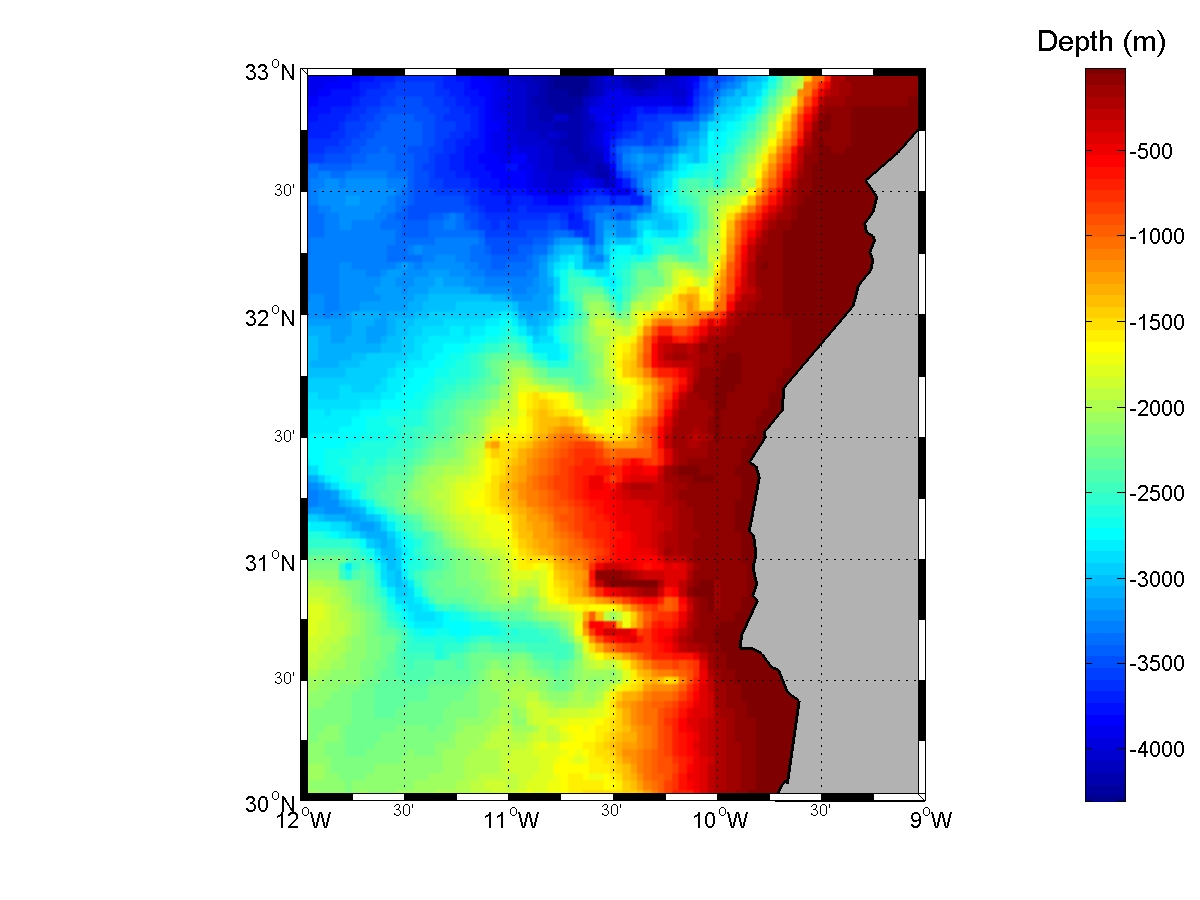
\includegraphics[width=.75\textwidth]{guir_topoNavy}
\caption{Topography from Naval Oceanographic Office website.\label{fig:topoNaval}}
\end{figure}


\subsection{Method 3: interpolation of individual topography measurements\label{sec:topotopex}}
%-------------------------------------------------------------------------

The principle of this method is to apply a \diva analysis to a data file containing depths at various locations.

\subsubsection{Get topography measurements}
%------------------------------------------

In the present example data points are extracted from \url{http://topex.ucsd.edu/cgi-bin/get_data.cgi} in the same region as the previous case ($9-12^{\circ}W\, \times\, 30-33^{\circ}N$). The output file is composed of three column: \texttt{| longitude | latitude | depth |}, i.e., the same format as \file{data.dat} files used by \diva. Once the file is downloaded, edit its name in \file{topo.dat}. Fig. \ref{fig:guirtopo} shows the individual measurements (coloured dots) in the region of interest. 


\begin{figure}[htpb]
\centering
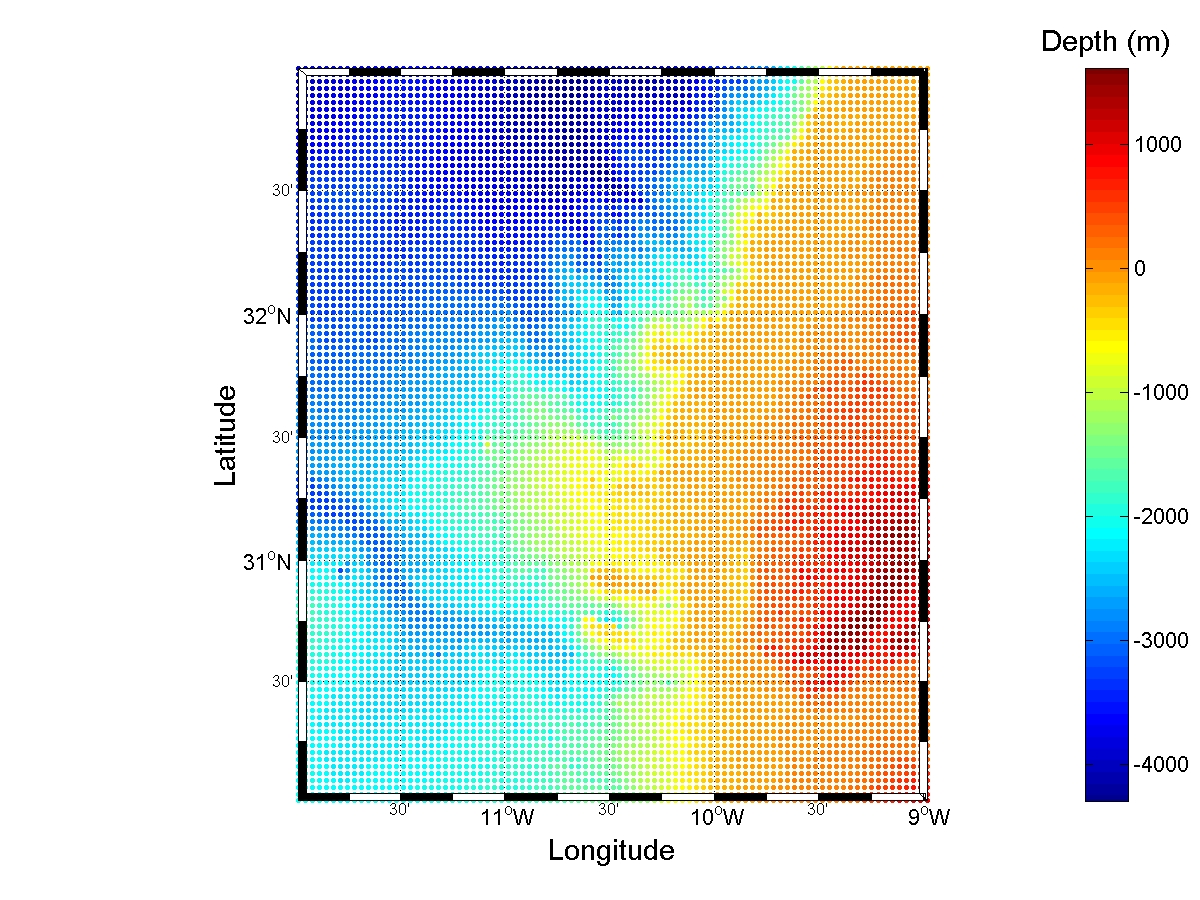
\includegraphics[width=.75\textwidth]{Ghir_topo_points}
\caption{Individual measurements of depths.\label{fig:guirtopo}}
\end{figure}


\subsubsection{Adapt parameters}
%-------------------------------

As in any \diva analysis, you need to provide parameters concerning the analysis itself and the output grid (file \file{param.par}, described extensively in Section~\ref{sec:param.par}, page \pageref{sec:param.par}). 

\begin{itemize}
\item Correlation length is chosen according to the resolution of the gridded topography you extracted, i.e., the distance between two measurements.
\item Signal-to-noise ratio is assigned with a large value (typically 100 or more).
\item \texttt{x/yorigin} are chosen according to the region where you extracted data.
\item \texttt{dx} and \texttt{dy} are the same as the values you use for your analysis. 
\end{itemize}



\subsubsection{Execute \command{divatopo}}
%----------------------------------------

With the two files \file{topo.dat} and \file{param.par} located in \directory{divastripped/input/}, type \command{divatopo} to launch the analysis. \command{divatopo} automatically creates a contour file according to grid parameters taken in \file{param.par}. The interpolated field is presented on Fig. \ref{fig:guirtopodiva}. Outputs \file{topo.grd} and \file{TopoInfo.dat} may then be used to generate contours (see Section~\ref{sec:contourgen}). 



\begin{figure}[htpb]
\centering
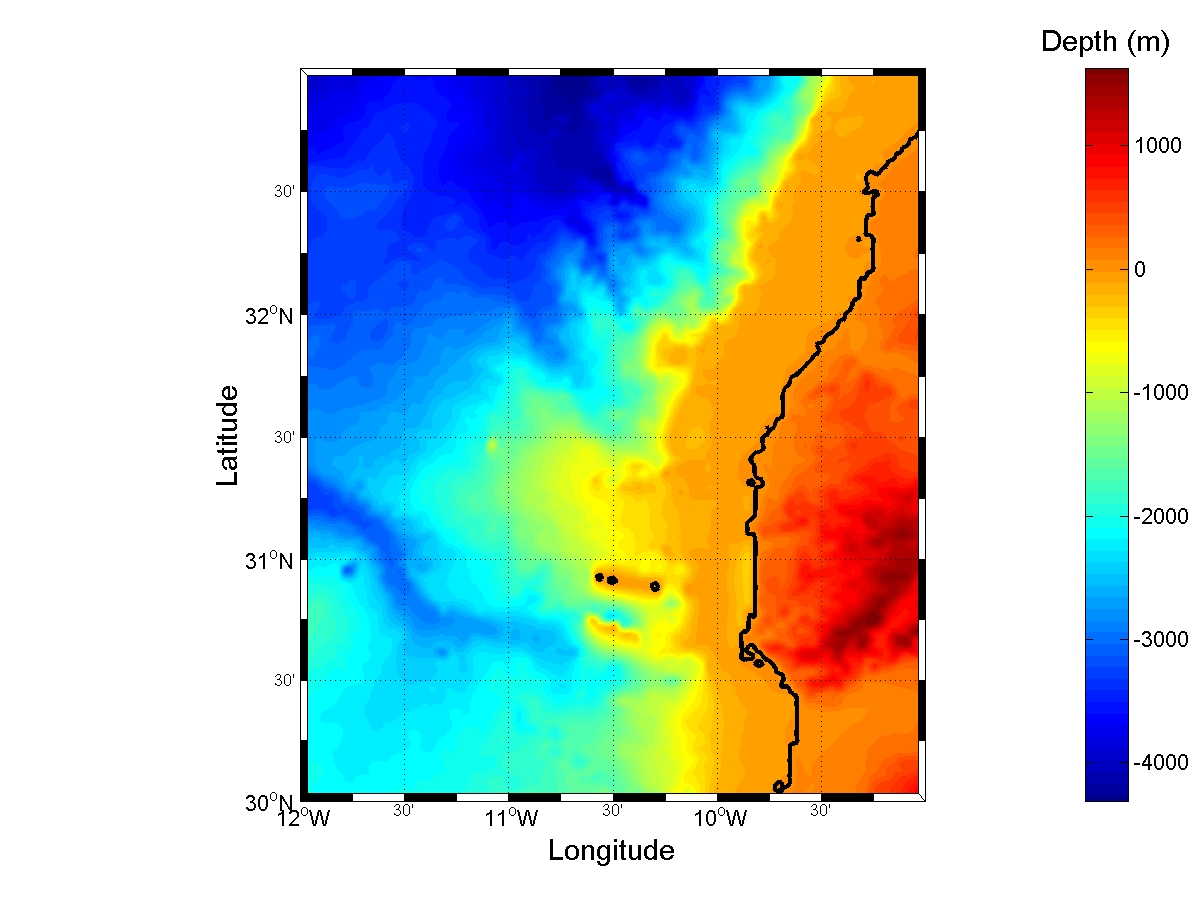
\includegraphics[width=.75\textwidth]{Ghir_topo_topex}
\caption{Interpolated topography.\label{fig:guirtopodiva}}
\end{figure}


\subsection{Method 4: by hand}
%----------------------

Create a gridded file (in the same format as the analysis fields \file{fieldgher.anl}) of topography and call
it \file{topo.grd}. The information on the grid's geographical dimensions are to be placed in \file{TopoInfo.dat}.

The grid is simply an array ($i=1,\ldots,M$) and ($j=1,\ldots,N$), where the coordinates of the grid nodes are
$x_i=x_1+(i-1)*dx$, $y_j=y_1+(j-1)*dy$.  The file \file{TopoInfo.dat} contains simply
\begin{verbatim}
x1
y1
dx
dy
M
N
\end{verbatim}


Look into \file{dvdv2diva.f} in \directory{./src/Fortran/Util/} how to write such files from within a Fortran code.


\section{Creation of contours\label{sec:contourgen}}
%-------------------------------------------------

\index{Contours}
As seen in first chapter, a relevant asset of \diva is the fact that it takes into account real coastlines and topography of the region of interest. We explain hereinafter the techniques to produce a correct coastline file, of which the description is provided in Section~\ref{contourdiva}.


\subsection{By hand}
%----------------------

The first possibility is to build your file \textit{by hand}: having at your disposal the location of different points of the coast (longitude, latitude), simply create a file containing $M$ contours, with the $i-th$ contour having being made up of $N_{i}$ points ($i=1,2,\ldots, N$). 

Be aware that some cases (Fig.~\ref{divaprob}) are to be avoided, since problems arise during the mesh generation when crossings occur in the contour. Also note that, as contours are automatically closed by \diva, the segment joining the first and the last points may generate errors. 


\begin{figure}[H]
\centering
\parbox{.5\textwidth}{
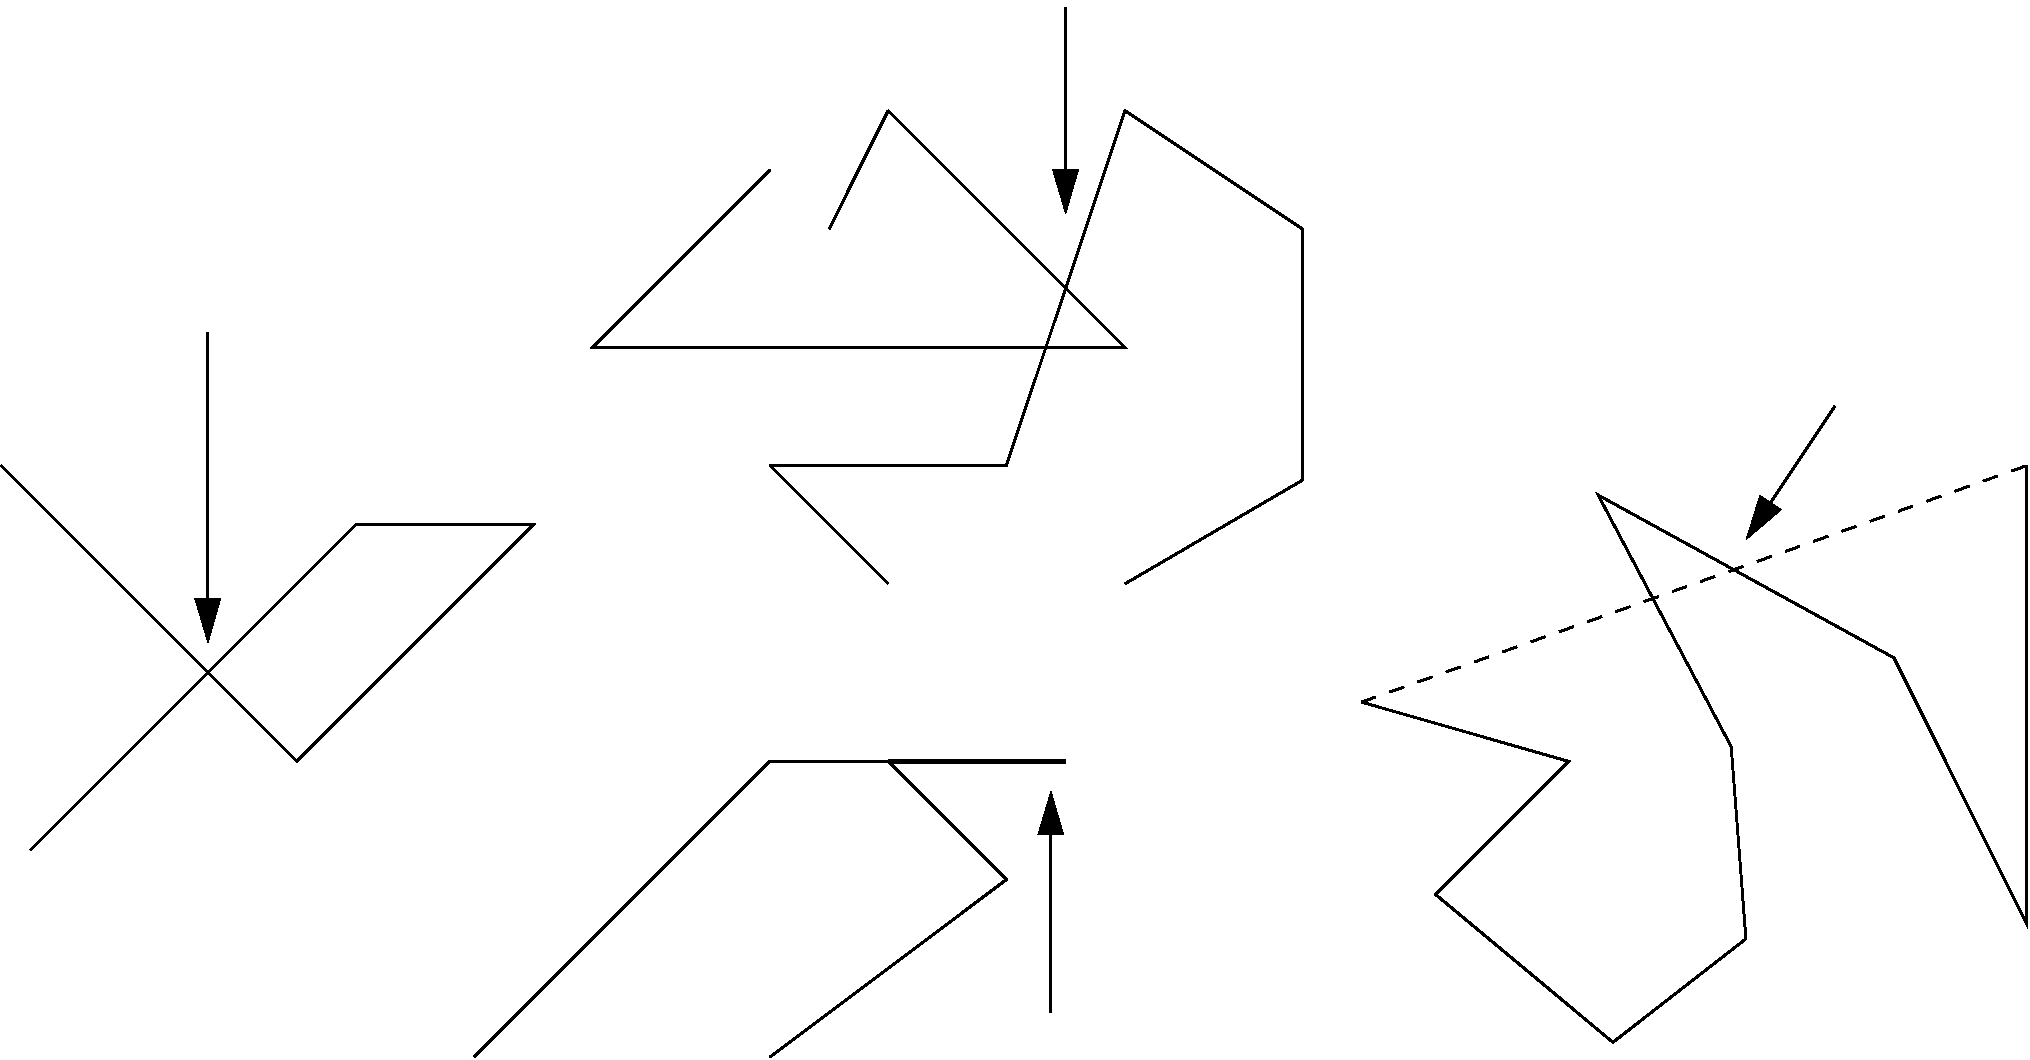
\includegraphics[width=.45\textwidth]{divaproblems}
}\parbox{.5\textwidth}{\caption[Example of improper contours.]{Example of improper contours. Left: crossing of two segments of a same contour; up: crossing of two different contours; right: first and last points of the contour generate a segment that crosses the other parts; down: two contours having a common segment.\label{divaprob}}
}
\end{figure}

Remember that you can use the tool \command{divacck} for checking and thinning of contours.


\subsection{From topography\label{sec:contourtopo}}
%--------------------------------------------------


Once you have placed files \file{topo.grd} and \file{TopoInfo.dat} in directory \directory{./input}, type \command{divacont} in the command line shell. This will generate several coastline files named \file{coast.cont.100nn}, where $nn$ corresponds to the $nn^{th}$ level defined in \file{contour.depth}. File \file{coast.cont} contains the coastline at the surface level ($z=0$).

As an illustration, we want to have contours from surface to a depth of \mbox{1000 m} every \mbox{200 m}, with \file{topo.grd} and \file{TopoInfo.dat} created in the Section~\ref{sec:howtotopo}. To this end we use the following file:

\begin{exfile}[htpb]
\begin{footnotesize}
\begin{verbatim}
2500
2000
1500
1000
500
0
\end{verbatim}
\end{footnotesize}
\caption{contour.depth\label{contourdepth}}
\end{exfile}

Contours for the specified depths are showed on Fig.~\ref{fig:contourdepth}.


\begin{figure}[htpb]
\centering
%\begin{tabular}{ccc}
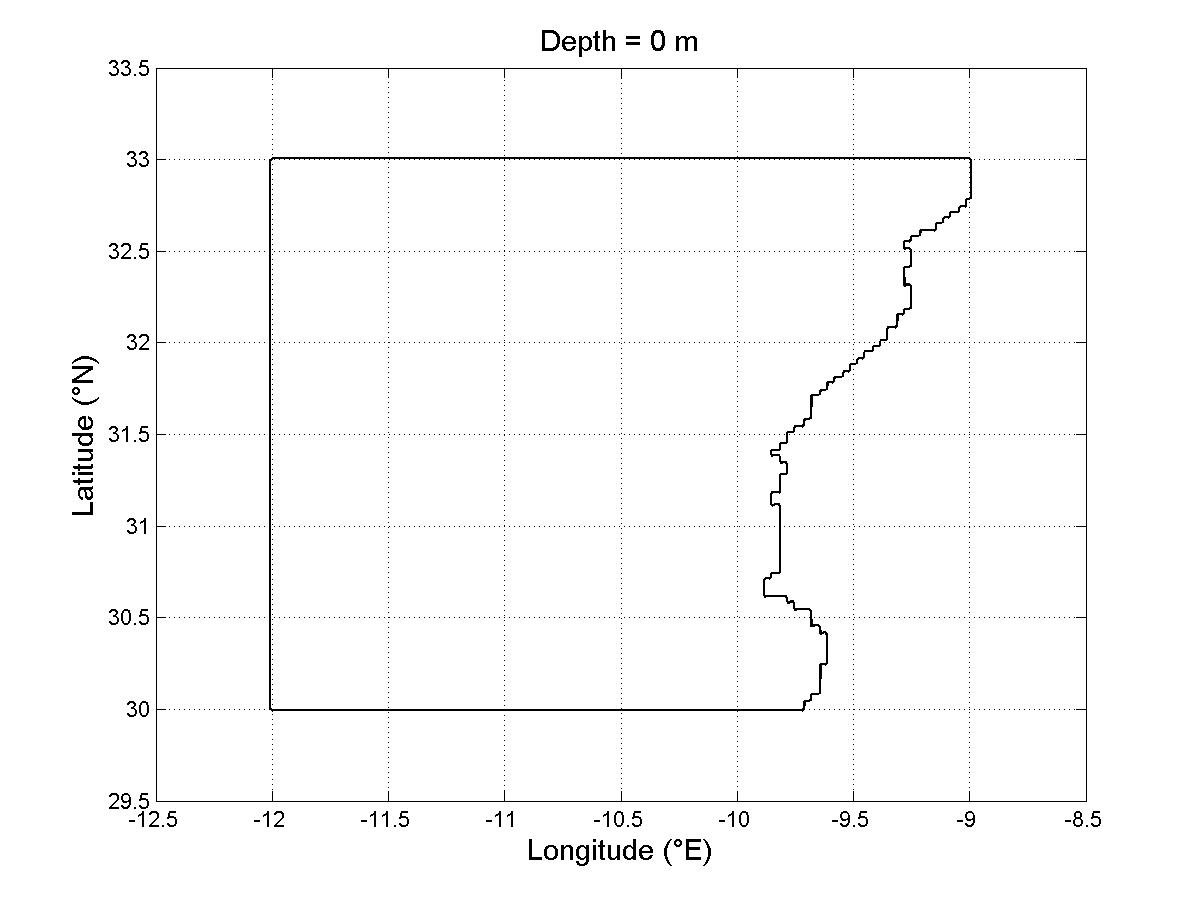
\includegraphics[width=.33\textwidth]{Ghir_contour_0}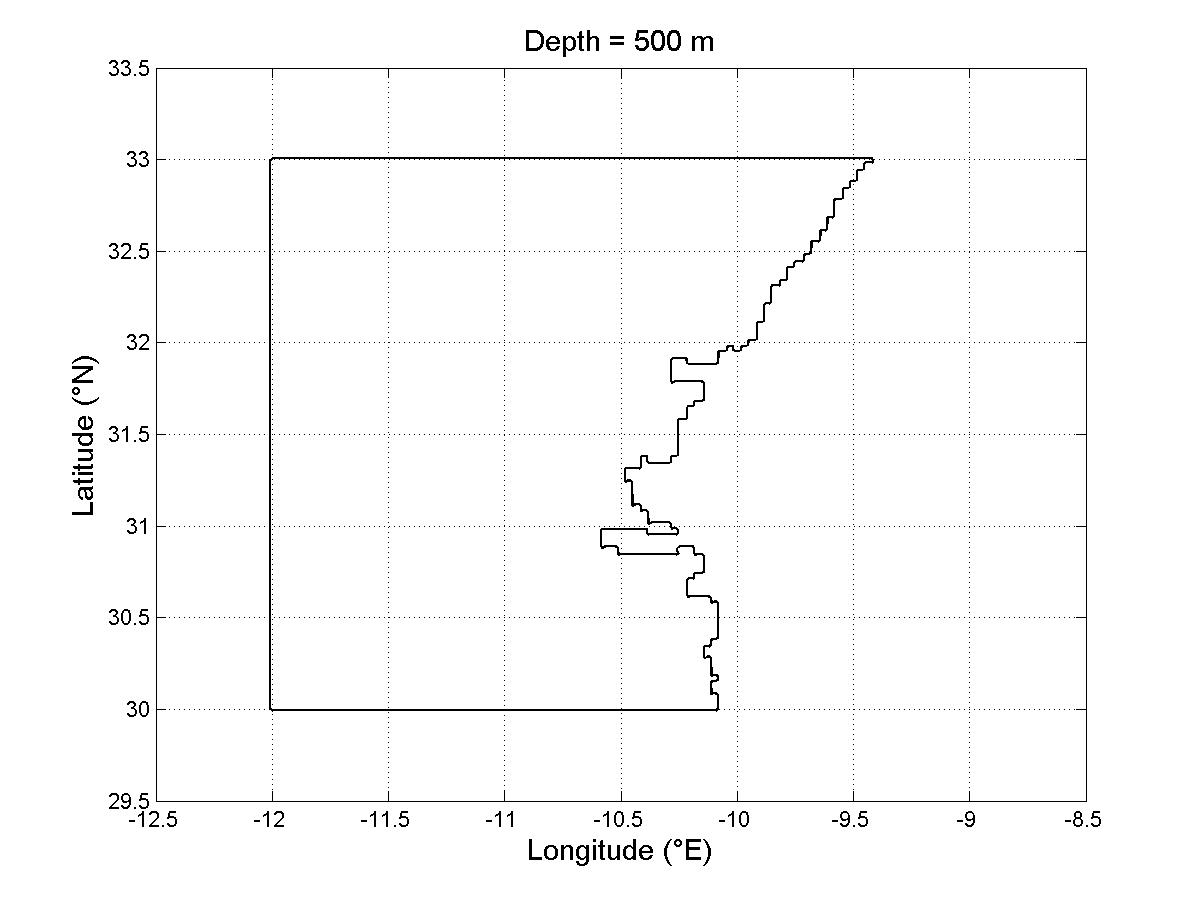
\includegraphics[width=.33\textwidth]{Ghir_contour_500}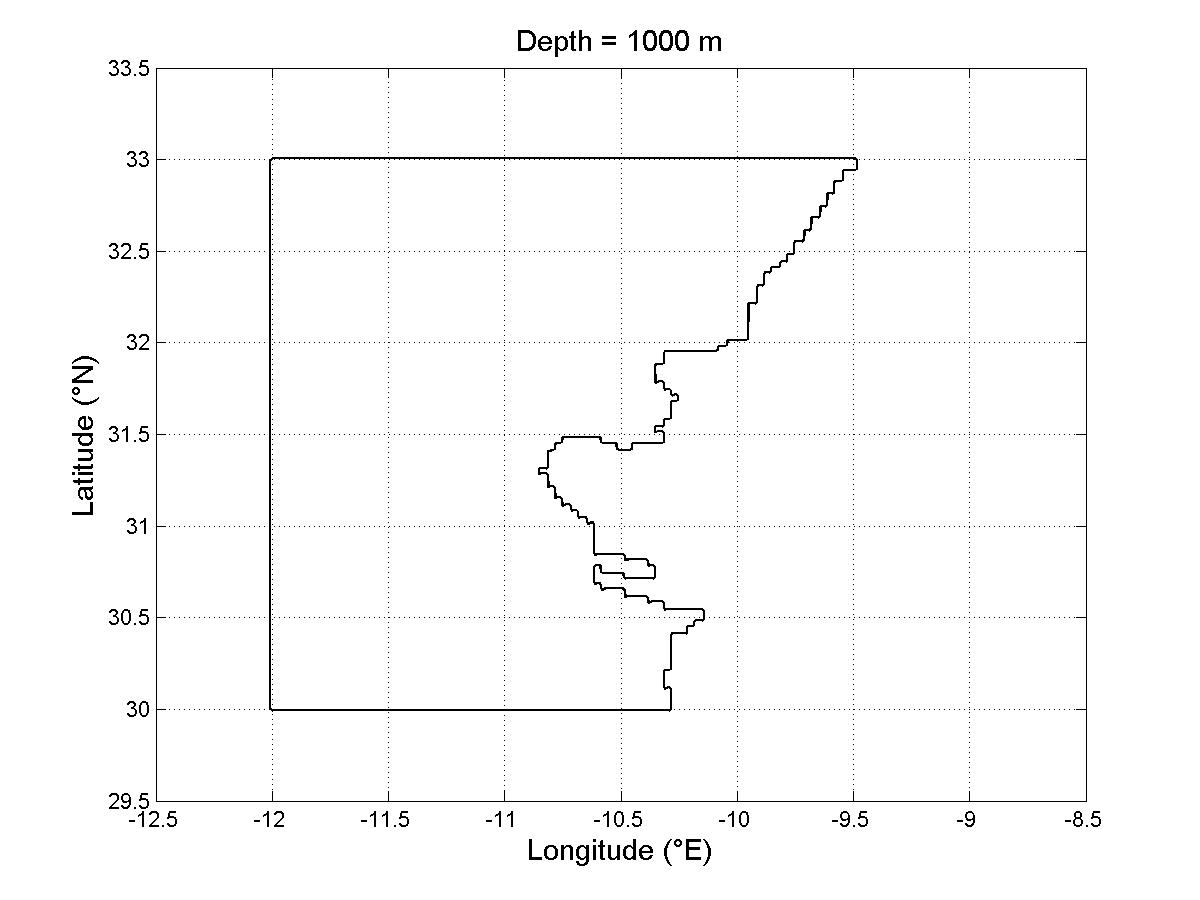
\includegraphics[width=.33\textwidth]{Ghir_contour_1000}\\
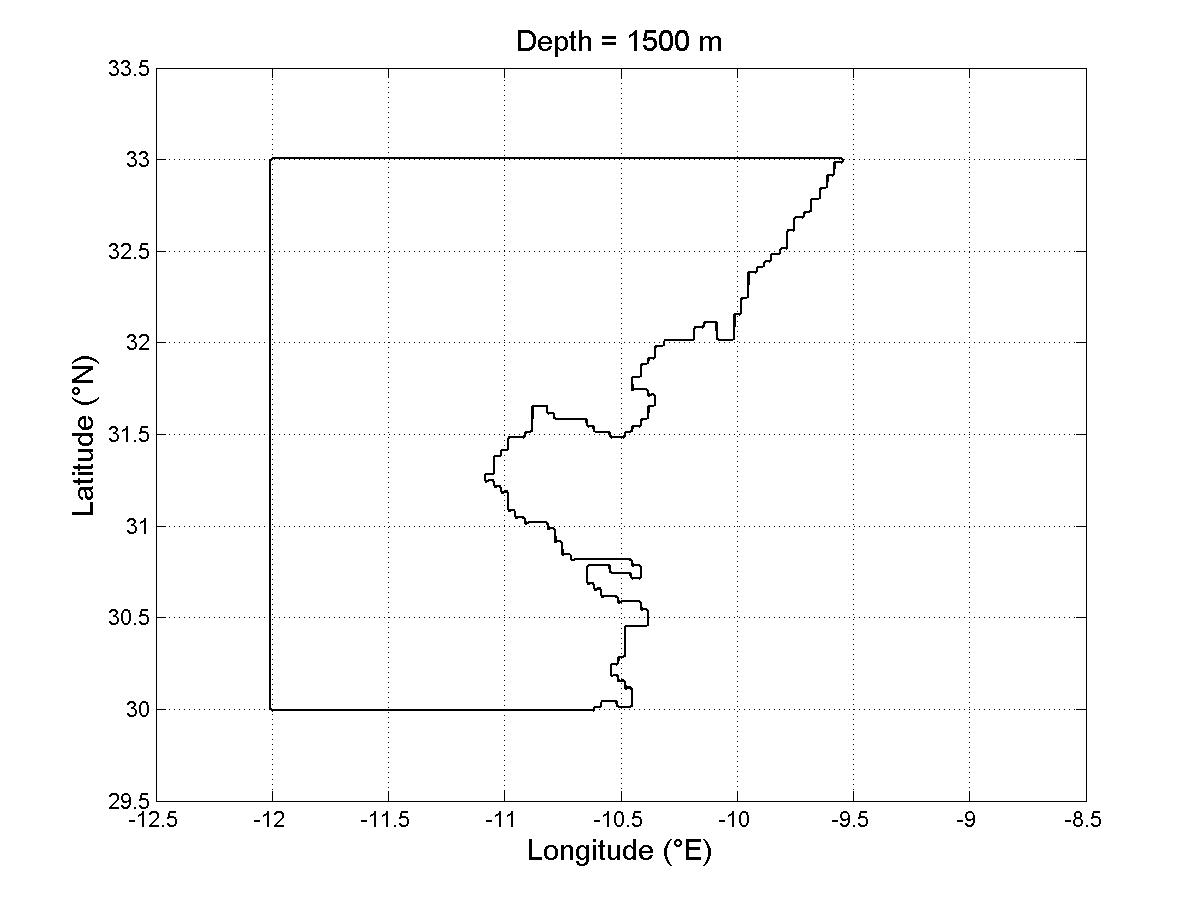
\includegraphics[width=.33\textwidth]{Ghir_contour_1500}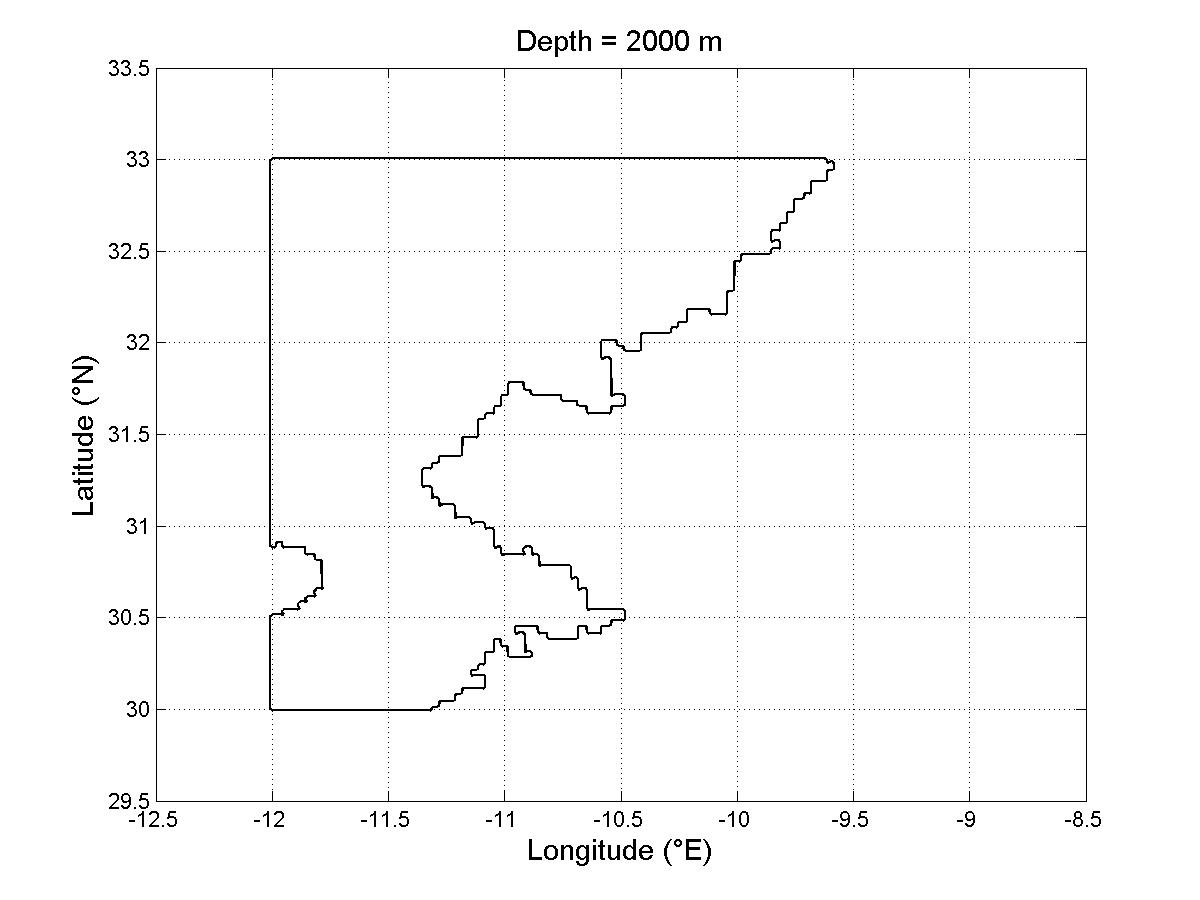
\includegraphics[width=.33\textwidth]{Ghir_contour_2000}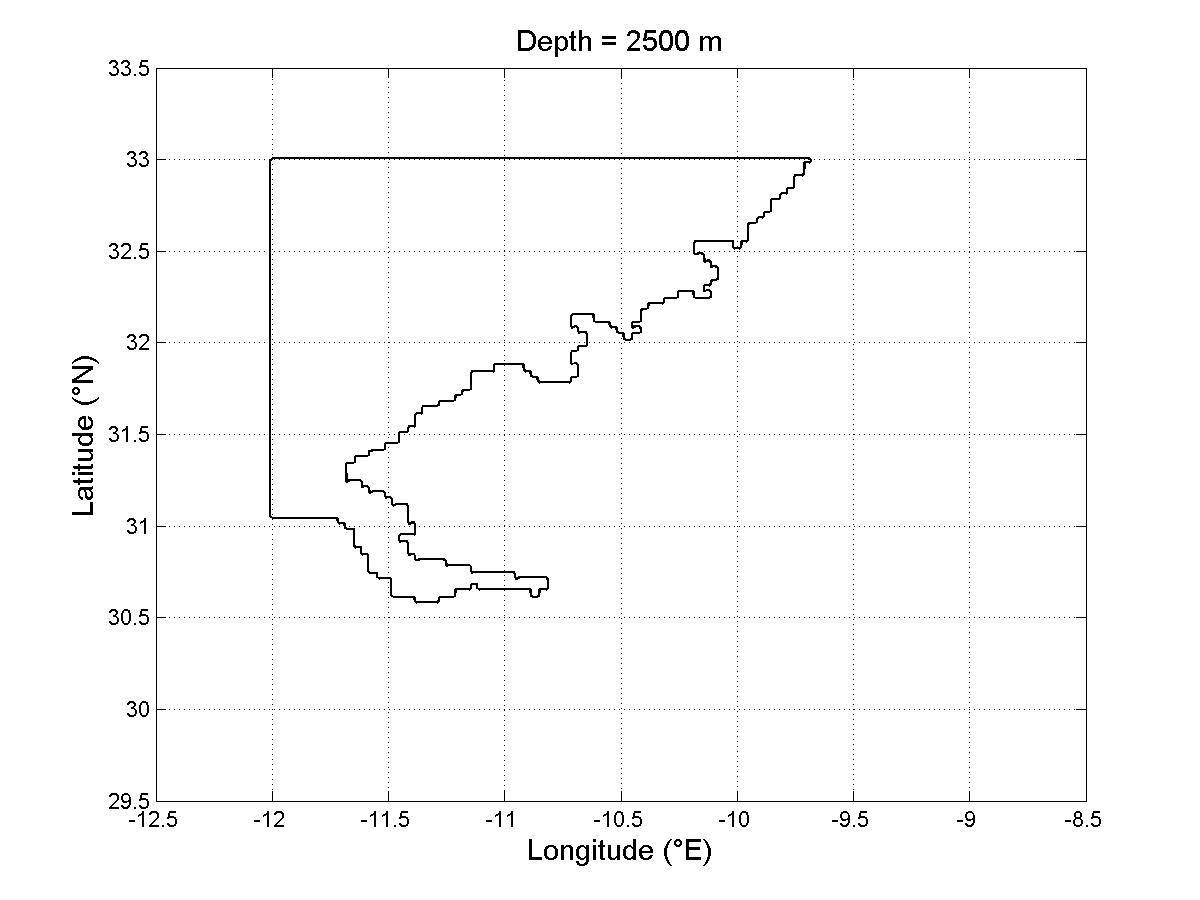
\includegraphics[width=.33\textwidth]{Ghir_contour_2500}

\caption{Contour generated every 500~m from surface to -2500~m.\label{fig:contourdepth}}
\end{figure}

\subsection{Using ODV}
%---------------------

\index{Ocean Data View}
Tool \command{divacoa2cont} allows converting ODV-format coastlines to \diva-format coastlines. Simply copy coastline file in the \directory{input} directory with the name \file{coast.coa} along with a \file{param.par} file and type \command{divacoa2cont} in the shell. 

This provides you the new file \file{./input/coast.cont}.



\subsection{From a mask}
%--------------------------

Simply look at \file{contourgen.f} and create the mask as you wish. Alternatively you can
create a pseudo-topography with adequate pseudo-depth at which you draw the contour.


%---------------------------------------------
\section{Determination of analysis parameters}
%---------------------------------------------

Two key parameters have to be adjusted before running an analysis: the correlation length ($L$) and the signal-to-noise ratio ($\snr$). Several tools are provided in order to help the user for the determination of these parameters.


\subsection{\command{divafit} \label{sec:divafit}}
%------------------------------------------------

\index{Correlation length}
The script \command{divafit}: uses the data (\file{./input/data.dat}) for a direct fitting of the covariance function (see Section~\ref{sec:kernel}). Note that the fit needs a sufficiently large data set.

\subsubsection{Command description}
%-----------------------------------------

\command{divafit} \qquad: performs a fit of the data correlation function based on the whole data set. \\
\command{divafit -r} \qquad: puts the new value of $L$ in \file{param.par} in function of the fit.\\
\command{divafit n} \qquad: performs the fit on a sample of \texttt{n*(n-1)/2} couples of data (sub-sampling). 

\example\\
\command{divafit -r 100}: performs a fit on $4950$ couples of data and update the file \file{param.par}.

\btips
When dealing with very large datasets, using \command{divafit} with sub-sampling may save you a large amount of time.
\etips

\textbf{Note:} when using advection constraint and variable $L$, \command{divafit} will not provide a very meaningful value.

\subsubsection{Output files}
%---------------------------

In output file \file{./output/paramfit.dat}, the best estimates are given and could be used as parameter values for running \diva.
Estimates of the correlation length are rather robust while those of the signal-to-noise ratio are neither precise nor robust, especially for large values.

Output file \file{covariance.dat} is the data-based covariance function:
\begin{description}
\item[column 1:] distance between points,
\item[column 2:] covariances, 
\item[column 3:] number of data couples used to estimate the covariance. 
\end{description} 

Output file \file{covariancefit.dat} allows looking at the fitted covariance function:
\begin{description}
\item[column 1:] distance between points, 
\item[column 2:] data-covariance, 
\item[column 3:] fitted covariance.
\end{description} 

Finally, file \file{param.par.fit} is the original \file{param.par} file except that the correlation length has been replaced by the fitted value. 

\textbf{Note:} always have a look at the fit to judge on its quality. %see example ref... divacovafit

\subsection{\command{divagcv}}
%-------------------------------

\index{Signal-to-noise ratio}\index{Generalised cross validation}
The script \command{divagcv} exploits \diva module (\texttt{gcvfac}), analysing random fields to assess the generalized cross validator (GCV, see Chapter~\ref{chap:analysisparameters} for theoretical developments). The script \command{divagcv} is an example of how to minimize the estimator by changing the signal-to-noise ratio ($\snr$) value, but could be adapted to optimize other parameters as well, such as correlation length.

Input to the module is the number of random estimates required (the larger the value, the more robust the estimator). Default value is 5, unless you change in \command{divacalc}. The user has to provide an input file \file{./input/gvcsampling.dat} containing the list of values for $\snr$ on which to try the estimator (typically around the values provided by \command{divafit}).

During the \command{divagcv} execution, error-field calculations are disabled to reduce computing time. 

\btips
If a mesh already exists (in \directory{meshgenwork} directory), \command{divagcv} disables the \command{divamesh} procedure. For this reason, ensure you are working with the adequate mesh.
\etips

\subsubsection{Output files}
%---------------------------

File \file{./output/gcv.dat} contains the GCV estimator:
\begin{description}
\item[column 1:] signal-to-noise ratio, 
\item[column 2:] GCV,
\item[column 3:] data anomaly variance.
\end{description}  
and \file{./output/gcvsnvar.dat} the best new estimate for the S/N and \texttt{VARBAK} parameters.

In \file{param.par.gcv}, you find an adapted version of the original \file{param.par}.



\subsection{\command{divacv}}
%-------------------------------

\command{divacv} carries out a cross validation, point by point, without new matrix inversions. 

\subsection{\command{divacvrand}}
%-------------------------------

\command{divacv} runs a cross validation by sub-samples of points.


Note that in the present version (\diva-\divaversion), tools  \command{divacv} and \command{divacvrand}  
do not adapt the error norm to include the relative weights on data. This will be introduced in the next versions.

%--------------
\section{Misc}
%--------------

\subsection{\command{divaclean}}
%-----------------------------

\command{divaclean} cleans up the working directories by removing \file{fort.*} files from \directory{divawork} and \directory{meshgenwork}, as well as output files from \directory{output}.

\subsection{\command{divadataclean}}
%-----------------------------

Script \command{divadataclean} takes the input data \file{./input/data.dat} and eliminates all data that fall outside the bounding box of the contours (i.e., the rectangle containing the analysis mesh). This avoids loading unnecessary large input files. If two additional arguments $n_{1}$ $n_{2}$ are added, data values falling outside the range specified by $n_{1},n_{2}$ are also eliminated.

\example
\begin{lstlisting}[style=Bash]
[charles@gher13 divastripped] divadataclean -3 35
\end{lstlisting}
will remove all data points of which the value is not between $-3$ and $35$.

The output overwrites \file{./input/data.dat} but keeps the original one in \directory{./input/} with the name \file{data.dat.full}. The tool should be used just after having loaded the data set (typically after \command{divaload}).

\subsection{\command{divaload}\label{sec:divaload}}
%--------------------------------------------------

\command{divaload} loads input files from the chosen directory into \directory{divastripped/input/}. You just have to specify the directory where your input files are located (relative or absolute paths). It is assumed that the input files are located in a folder \directory{input} within the chosen directory.

\example
\begin{lstlisting}[style=Bash]
[charles@gher13 divastripped] divaload ~/DIVA/test/
\end{lstlisting}
will load the files from \directory{\textasciitilde/DIVA/test/input}.
 

\btips
When you want to know to which correspond the data present in the input directory, simply read the content of the file \file{input/casename}; it indicates the repertory from which you loaded input files with command \command{divaload}.
\etips


\subsection{\command{divacck}}
%-----------------------------

\index{Contours}
\command{divacck} checks your initial contour file \file{./output/coast.cont}. In output \file{./\-output/\-coast.cont\-.checked} you will find a thinned contour based on the length scale, where the possible couples of identical points are eliminated.

Application of \command{divacck} is normally not necessary if you created the contours with \command{divacont}.
